\chapter{CH PLIF Signal Modeling and Validation}
\label{ch:chplif}

% This chapter covers the modeling of the CH PLIF signal and contains the following sections:

% 0. Preliminary experiments
%   0.1 Excitation scan
%   0.2 Linearity test
% 1. Signal modeling
%     1.1 Constants, assumptions, simplifications
%     1.2 Comparison of models (GRI, USCv2, Syngas, C1-C3, San Diego, etc.) / CH₄+air results
% 2. Results
%   Unstrained, laminar flames
%     2.1 Methane + air flames
%         2.1.1 subsection comparison with experiments
%     2.2 C1-C3 alkanes flames
%     2.3 Syngas mixtures
%     2.4 Syngas + C1-C3 alkanes
%   Strained laminar flames
%     2.5 Strain effects

% Questions to be answered (from proposal):

% 1. Detailing the development of a CH PLIF system (covered in Chapter 2,3 and here)
% 2. Demonstration on an atmospheric pressure laminar flame
% 3. Validate with quenching models
% 4. Model signal for strained flames
% 5. Model signal for fuel mixtures

% TODO:Write a short introduction to the chapter to start it off

\section{CH PLIF Preliminary Experiments}
\label{sec:chplif-preliminary-experiments}

The CH PLIF imaging system was evaluated for use in imaging hydrocarbon flames by performing two preliminary experiments.
First, an excitation scan was performed to confirm the location of the optimal wavelength to excite the CH radicals in a typical hydrocarbon flame.
Second, a test of the linearity of the LIF signal with respect to the incident laser intensity was performed.
The setup and results of these experiments are described in the following subsections.

\subsection{Excitation Scan}
\label{subsec:prelim-excitation-scan}

\begin{figure}

\centering

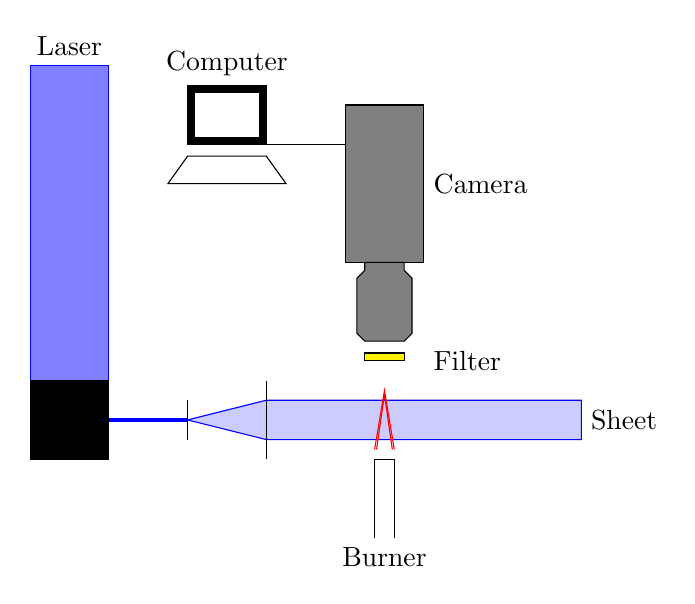
\begin{tikzpicture}

% Laser
\filldraw [fill=blue!50!white, draw=blue] ( 0, 5 ) rectangle ++( 1, -4 );
\filldraw [black] ( 0, 1 ) rectangle ++( 1, -1 );

% Beam
\draw [very thick, blue] ( 1, 0.5 ) -- ++( 1, 0 );
\draw [draw=blue,fill=blue!20!white] ( 2, 0.5 ) -- ++( 1, 0.25 ) -- ++( 4, 0 ) -- ++( 0, -0.5 ) -- ++( -4, 0 ) -- cycle;

% Lenses
\draw ( 2, 0.25 ) -- ++( 0, 0.5 );
\draw ( 3, 0 ) -- ++( 0, 1 );

% Laminar burner
\draw ( 4.375, -1 ) -- ++( 0, 1 ) -- ++( 0.25, 0 ) -- ++( 0, -1 );

% Flame
\draw [red] ( 4.375, 0.125 ) -- ++( 0.125, 0.75 ) -- ++( 0.125, -0.75 );
\draw [red] ( 4.4, 0.125 ) -- ++( 0.1, 0.7 ) -- ++( 0.1, -0.7 );

% Camera
\filldraw [fill=black!50!white, draw=black] ( 4, 4.5 ) rectangle ++( 1, -2 );
\filldraw [fill=black!50!white, draw=black] ( 4.25, 2.5 ) -- ++( 0, -0.1 ) -- ++( -0.1, -0.1 ) -- ++( 0, -0.7 ) -- ++( 0.1, -0.1 ) -- ++( 0.5, 0 ) -- ++( 0.1, 0.1 ) -- ++( 0, 0.7 ) -- ++( -0.1, 0.1 ) -- ++ ( 0, 0.1 ) -- cycle;

% Filter
\filldraw [fill=yellow, draw=black] ( 4.25, 1.25 ) rectangle ++( 0.5, 0.1 );

% Computer
\filldraw [black] ( 2, 4 ) rectangle ++( 1, 0.75 );
\filldraw [white]( 2.1, 4.1 ) rectangle ++( 0.8, 0.55 );
\draw ( 2, 3.85 ) -- ++( 1, 0 ) -- ++( 0.25, -0.35 ) -- ++( -1.5, 0 ) -- cycle;

\draw ( 3, 4 ) -- ++( 1, 0 );

% Labels
\node at ( 0.5, 5 ) [above] {Laser};
\node at ( 2.5, 4.75 ) [above] {Computer};
\node at ( 5, 3.5 ) [right] {Camera};
\node at ( 5, 1.25 ) [right] {Filter};
\node at ( 4.5, -1 ) [below] {Burner};
\node at ( 7, 0.5 ) [right] {Sheet};

\end{tikzpicture}

\caption[Schematic of the excitation scan experiment]{The figure above shows the schematic of the excitation scan experiment. Optics form the laser beam into a collimated sheet focused over a laminar Bunsen burner. The fluorescence is imaged perpendicularly by an intensified camera synchronized to the laser pulse. A 3 mm GG 420 filter is used to reject elastic scattering.}

\label{fig:excitationScan}

\end{figure}



An excitation scan is performed by tuning the output of the alexandrite laser from \(\lambda\) = 387.077 nm to 387.260 nm.
This serves two purposes.
First, it locates the optimal wavelength to excite the CH radicals that results in the highest fluorescence yield.
Second, the variation of the signal intensity can be compared with simulated profiles from LIFBASE or other spectroscopic calculations and our estimation of the laser linewidth can be validated.
The laser linewidth is an integral parameter and appears in the absorption integral used by the models developed in Chapter \ref{ch:background}.

A schematic of the excitation scan experiment is shown in Figure \ref{fig:excitationScan}.
The intensified PI Acton 512\(\times\)512 camera described in Section \ref{subsec:experimental-ch-chemiluminescence} is used to image a premixed, laminar methane-air flame operating at close to stoichiometric conditions.
The laminar flame is stabilized on the Bunsen burner described in Section \ref{subsubsec:plif-laminar-flame-setup}.
The alexandrite laser is operated at a power of 16 mJ/pulse in the second harmonic.
The sheet forming optics consist of a +50 mm cylindrical lens and a +250 mm spherical lens placed 300 mm apart.
The optics form the beam into a collimated sheet about 25 mm (1 in) tall, focused to a thickness on the order of 250 \(\mu\)m at the flame location.
The sheet passes through the center of the flame and the edges of the sheet are blocked by razor blades to prevent reflections from the burner from saturating the camera.

The induced fluorescence in the flame sheet is imaged perpendicularly by the intensified camera using an 85 mm f/1.8 Nikon AF Nikkor lens.
A 3 mm thick 50 mm\(\times\)50 mm square GG 420 Schott glass filter is used to reject elastic scattering at the excitation wavelength.
This setup gives a magnification of approximately 62 \(\mu\)m/pixel.
The camera is triggered by the flash lamp sync signal from the laser system and the intensifier is gated over 300 ns, encompassing the 70 ns laser pulse.
The long gate width gives the intensifier enough time to prepare to receive the fluorescence, preventing signal loss due to irising.
The gate width is still short enough that minimal flame chemiluminescence or ambient lighting is recorded in the images.
100 instantaneous images are acquired for each excitation wavelength to acquire a good estimate of the mean fluorescence signal, \(\mu_{sig}\).

Figure FIXME shows a sample CH PLIF image from this dataset.
The images are background-corrected by subtracting the laser scattering (recorded without the flame).
The fluorescence signal is calculated from these images using three alternate approaches.

In Method I, two ``windows'' are identified that include the straight sections of the laminar flame.
The average fluorescence signal in each frame is calculated by taking the average of all the emitting pixels in the two windows.
A pixel is designated as an emitting pixel if its intensity exceeds the standard deviation of a typical background pixel by at least a factor of five.
The average of this value over all the frames is designated as the mean fluorescence signal, \(\mu_{sig}\).
In Method II, the intensity of the pixels is integrated over a straight line connecting the inner and outer edges of the flame.
The straight line is chosen along the beam so that the beam intensity does not vary along the integration path.
The integration is performed on the left and right arms of the flame, giving two readings per frame.
The mean of these values over all the frames is recorded as the mean fluorescence signal, \(\mu_{sig}\).
In Method III, the midpoints of the straight lines from Method II are located and the average of their intensities, over all the frames is recorded as the mean fluorescence signal, \(\mu_{sig}\).
The regions of interest for each of these methods is highlighted in Figure FIXME.

The result of this investigation is shown in Figure FIXME.
The calculated mean fluorescence signals from the three methods are plotted against a LIFBASE simulation of the absorption spectrum of the CH \(B-X\) transition.
The profiles are appropriately scaled to match the LIFBASE simulation at the maximum value and at the minimum value.
The LIFBASE simulation is performed for a thermalized system at 1800 K, at atmospheric pressure.
Further, the instrument linewidth is specified to be the same as our estimate of the laser linewidth (1.06 \AA).

The profiles of the calculated and scaled mean fluorescence signals are observed to agree extremely well with the LIFBASE simulation result.
The discrepancies between the three methods is minimal.

The results indicate that the optimal excitation wavelength, corresponding to the highest mean fluorescence signal, is about 387.2 nm.
For the rest of the experiments performed in this work, the laser is operated at this wavelength.
The results also help verify that the calibration of the micrometer is accurate and the wavelengths are precisely adjustable.
Finally, the results validate that our estimated laser linewith, 1.06 \AA, is accurate.
This value can now be used in subsequent calculations of the LIF signal levels.

\subsection{Linearity Test}
\label{subsec:prelim-linearity-test}

As explained in Chapter \ref{ch:background}, the variation of the fluorescence signal with the excitation laser intensity exhibits a saturation curve.
For reasons mentioned in that discussion, we prefer to operate in the weak excitation limit.
Further, the models developed in Chapter \ref{ch:background} for calculating the signal are intended to be used in the linear regime.
Hence, an experiment is performed to verify the linearity of the system response at the intensities at which the flames are imaged for this work.
The schematic of the setup is shown in Figure FIXME.
The laser is tuned to the optimal wavelength as determined in Section \ref{subsec:prelim-excitation-scan}, and operated at 10 Hz.
The frequency-doubled beam is directed at a steady, laminar, methane-air Bunsen flame operating at a slightly rich stoichiometry.
The edges of the beam are clipped by an aperture to produce a sharp edge and to avoid unnecessary reflections from the burner.
No optics are used to refract the beam in any way.

The flame is imaged by the PI Acton 512\(\times\)512 intensified camera equipped with a 50 mm, f/1.8 AF Nikkor lens.
Elastic scattering is attenuated by a 3 mm thick GG 420 Schott glass filter.
The magnification achieved by this set up is about 44 \(\mu\)m/pixel.
The LIF signal from the flame is recorded in 300 ns gates and accumulated 150 times before being read out.
For each case, a corresponding laser scattering image is also recorded for estimating the background.
The flame chemiluminescence and ambient background are also recorded for the same purpose.

For this experiment, varying the intensity of the laser beam by changing the flash lamp voltage or even the Q-switch timing is not preferred as either would alter the pulse width of the beam.
Instead, quartz disks and blocks of varying thickness are introduced into the beam to produce an intensity loss, while preserving all other characteristics of the beam.
The quartz elements decrease the intensity of the laser beam through reflection, scattering and absorption.
The stray reflections and scattering from the quartz elements are contained by enclosing the elements in a box and preventing these from being recorded by the camera.
In this manner, the laser power is varied from 10 mJ/pulse to 0.5 mJ/pulse and back.

The acquired images are background-corrected and the intensity is conditionally averaged over pixels with a non-zero intensity in the region where the fluorescence occurs.
The average fluorescence intensity values thus obtained are plotted against the corresponding laser intensity and shown in Figure FIXME.
A sample image highlighting the region of interest is also shown alongside.

The LIF signal is observed to increase monotonically with increasing laser intensity.
At the lower intensities, the variation is very nearly linear, with marginal scatter and only one significant outlier.
At intensities above 1 J/cm\(^2\) however, there is significant scatter in the data and the linear trend obtained from the low intensity cases cannot be reliably extended over this region.

The results indicate that as long as the intensity of the laser sheet is kept below 1 J/cm\(^2\), the assumption of operating in the linear regime is valid.

\section{Fluorescence Signal Modeling}
\label{sec:chplif-fluorescence-signal-modeling}

Chapter \ref{ch:background} presented analysis of LIF signal calculation as a function of thermodynamic conditions and the local composition in a flame.
Expressions derived using a basic model (Equation \ref{eqn:twoLevelModel}) and a more complex model (Equation \ref{eqn:improvedModel}) were presented.
The expressions rely on knowledge of several physical values and specific spectroscopic constants pertaining to the CH system.

\begin{table}
  \caption[Einstein A coefficients]{The coefficients of spontaneous emission for transitions in the CH system are provided.}
  \begin{center}
    \begin{tabular}{lcr}
      Transition & Symbol & A, s\(^{-1}\) \tabularnewline
      \hline\hline
      \(B\rightarrow X(0,0)\) & \(A_{20}\) & \(2.963 \times 10^6\) \tabularnewline
      \(A\rightarrow X(1,1)\) & \(A_{10}\) & \(1.676 \times 10^6\) \tabularnewline
      \(A\rightarrow X(0,0)\) & \(A'_{10}\) & \(1.832 \times 10^6\) \tabularnewline
    \end{tabular}
  \end{center}
  \label{tab:emissionCoefficients}
\end{table}


The basic model requires us to know the Einstein coefficient for spontaneous emission from the ``upper'' state to the ``lower'' state.
For this, we assume that the ``upper'' state has the same properties as the \(A^2\Delta\), \(v = 0\) state.
The improved model, needs the emission coefficients for the \(B^2\Sigma^-\), \(v = 0\) and \(A^2\Delta\), \(v =\) 0, 1 states.
These are tabulated from sources in literature\cite{1985-garland-a,1996-luque-b} FIXME in Table \ref{tab:emissionCoefficients}.

\begin{table}
  \caption[Quenching Cross-sections]{The functional form of the quenching cross-sections of various species with CH are provided.}
  \begin{center}
    \begin{tabular}{lr}
      Species & \(\sigma\), \AA\(^2\) \tabularnewline
      \hline\hline
      \ce{H2} & \(6.1 \exp{ \left(-686 / T \right)}\) \tabularnewline
      \ce{H} & \(221 T^{-0.5} \exp{ \left( -686 / T \right)}\) \tabularnewline
      \ce{O2} & \(8.61 \times 10^{-6} T^{1.64} \exp{ \left( 867 / T \right)}\) \tabularnewline
      \ce{OH} & \(221 T^{-0.5} \exp{ \left( -686 / T \right)}\) \tabularnewline
      \ce{H2O} & 9.6 \tabularnewline
      \ce{CH4} & \(52.8 T^{-0.5} \exp{ \left( -84 / T \right)}\) \tabularnewline
      \ce{CO} & 8.31 \tabularnewline
      \ce{CO2} & \(8.67 \times 10^{-13} T^{3.8} \exp{ \left( 854 / T \right)}\) \tabularnewline
      \ce{C2H6} & 13.4 \tabularnewline
      \ce{N2} & \(1.53 \times 10^{-4} T^{1.23} \exp{ \left( -522.1 / T \right)}\) \tabularnewline
      \ce{C3H8} & 22 \tabularnewline
      \hline
    \end{tabular}
  \end{center}
  \label{tab:quenchingCrossSections}
\end{table}



Next, to calculate the fluorescence yield for the basic model, we need to know the quenching cross-sections of major species found in the flames of interest.
These cross sections are curve-fitted from several experiments performed over varying ranges of temperature.
The functional forms of these cross-sections are presented in Table \ref{tab:quenchingCrossSections}.

The fluorescence yield expressions for the complex model require the rates of collisional transfer between several energy levels.
There have been efforts to measure and model these rates, but the energy level model used for these studies is more complicated and cannot be easily reconciled with our simplified model.
Hence, it would be preferable to make some simplifying assumptions so that the collisional rates can be reduced in terms of the quenching rate.

Previous work has reported that the rate of quenching does not appreciably vary over the vibrational manifold, but excited CH molecules in the \(B^2\Sigma^-\) electronic state are approximately 30\% more likely to be quenched than molecules in the \(A^2\Delta\) states.
This allows us to eliminate \(Q'_{10}\) and \(Q_{20}\) as follows.

\begin{gather}
  Q'_{10} = Q_{10} = Q
  \label{eqn:quenchingAssumption1}\\
  Q_{20} = 1.3Q
  \label{eqn:quenchingAssumption2}
\end{gather}

Our next assumption is based on work by Luque et al.\cite{2000-luque} FIXME who reported that the rate of transfer following the \(B^2\Sigma^-\rightarrow A^2\Delta\) (0,1) transition accounts for almost 24\% of the collisional removal of CH from the upper electronic state.
This allows us to formulate one more equation as shown below.

\begin{gather}
  \frac{ Q_{21} + Q'_{21} - Q_{12} }{ Q_{20} + Q_{21} + Q'_{21} - Q_{12} } = 0.24\\
  \therefore \frac{ R_{21} + R'_{21} - R_{12} }{ Q } = 0.4105
  \label{eqn:QEquation1}
\end{gather}

Next, using the reported results from the same authors\cite{2000-luque} FIXME, we know that the number of CH molecules following the \(B^2\Sigma^-\rightarrow A^2\Delta\) (0,1) transition is four times as much as the number following the \(B^2\Sigma^-\rightarrow A^2\Delta\) (0,0) transition.

\begin{equation}
  \frac{ Q_{21} - Q_{12} }{ Q'_{21} } = 4
  \label{eqn:QEquation2}
\end{equation}

Finally, Garland et al.\cite{1985-garland-b} FIXME reported that the rate of the forward transfer along the \(B^2\Sigma^-\rightarrow A^2\Delta\) (0,1) transition is about 60\% faster than the reverse process.

\begin{equation}
  \frac{Q_{21}}{Q_{12}} = 1.6
  \label{eqn:QEquation3}
\end{equation}

This gives us the third equation forming a closed, linear set of equations in terms of \(Q_{21}\), \(Q_{12}\) and \(Q'_{21}\) that can be written out in matrix form and solved.
Equation \ref{eqn:QSolution} presents the solution.

\begin{equation}
  \left[
    \begin{matrix}
      R_{21}\\
      R'_{21}\\
      R_{12}
    \end{matrix}
  \right] = \left[
   \begin{matrix}
      5.1966\\
      0.4872\\
      3.2479
    \end{matrix}
  \right] Q
  \label{eqn:QSolution}
\end{equation}

Substituting Equations \ref{eqn:quenchingAssumption1}, \ref{eqn:quenchingAssumption2} and \ref{eqn:QSolution} into Equations \ref{eqn:fluorescenceYield1-unsimplified}--\ref{eqn:fluorescenceYield2-unsimplified} leads to simplified expressions for the two fluorescence yields.
More importantly, they are now functionally dependent on only the Einstein coefficients and the rate of collisional quenching.

\begin{align}
  Y_1 &= \frac{ 5.1966Q }{ ( A_{10} + 4.2479Q )( A_{20} + 6.9838Q ) - 16.8780Q }
  \label{eqn:fluorescenceYield1}\\
  Y'_1 &= \frac{ 0.4872Q( A_{10} + 4.2479Q ) }{ ( A'_{10} + Q ) \left( ( A_{10} + 4.2479Q )( A_{20} + 6.9838Q ) - 16.8780Q \right) }
  \label{eqn:fluorescenceYield2}
\end{align}

\begin{table}
  \caption[Absorption lines and coefficients for the \(B^2\Sigma^-\leftarrow X^2\Pi\) (0,0) R branch]{The line positions and the corresponding Einstein coefficients for stimulated absorption for transitions in the \(B^2\Sigma^-\leftarrow X^2\Pi\) (0,0) R branch are presented below.}
  \begin{center}
    \begin{tabular}{lcccccc}
      \(N''\) & \(J''_1\) & \(\nu_1\) & \(B\) & \(J''_2\) & \(\nu_2\) & \(B\) \tabularnewline
        & & cm\(^{-1}\) & \(\times10^{-9}\) m\(^2\)J\(^{-1}\)s\(^{-1}\) & & cm\(^{-1}\) & \(\times10^{-9}\) m\(^2\)J\(^{-1}\)s\(^{-1}\) \tabularnewline
      \hline\hline
      & & & & & & \tabularnewline
      1  & 0.5  & 25756.08 & 6.511 & 1.5  & 25774.03 & 5.823 \tabularnewline
      2  & 1.5  & 25776.42 & 7.225 & 2.5  & 25782.72 & 6.489 \tabularnewline
      3  & 2.5  & 25792.74 & 7.532 & 3.5  & 25797.06 & 7.174 \tabularnewline
      4  & 3.5  & 25805.42 & 7.671 & 4.5  & 25808.75 & 7.460 \tabularnewline
      5  & 4.5  & 25814.47 & 7.719 & 5.5  & 25817.20 & 7.581 \tabularnewline
      6  & 5.5  & 25819.80 & 7.708 & 6.5  & 25822.13 & 7.610 \tabularnewline
      7  & 6.5  & 25821.28 & 7.652 & 7.5  & 25823.32 & 7.581 \tabularnewline
      8  & 7.5  & 25818.72 & 7.561 & 8.5  & 25820.55 & 7.506 \tabularnewline
      9  & 8.5  & 25811.93 & 7.439 & 9.5  & 25813.59 & 7.396 \tabularnewline
      10 & 9.5  & 25800.64 & 7.288 & 10.5 & 25802.17 & 7.254 \tabularnewline
      11 & 10.5 & 25784.57 & 7.111 & 11.5 & 25785.98 & 7.083 \tabularnewline
      12 & 11.5 & 25763.38 & 6.907 & 12.5 & 25764.70 & 6.884 \tabularnewline
      13 & 12.5 & 25736.65 & 6.676 & 13.5 & 25737.88 & 6.657 \tabularnewline
      14 & 13.5 & 25703.90 & 6.418 & 14.5 & 25705.06 & 6.402 \tabularnewline
      15 & 14.5 & 25664.54 & 6.129 & 15.5 & 25665.64 & 6.116 \tabularnewline
      16 & 15.5 & 25617.87 & 5.815 & 16.5 & 25618.92 & 5.804 \tabularnewline
      17 & 16.5 & 25563.03 & 5.472 & 17.5 & 25564.03 & 5.463 \tabularnewline
      18 & 17.5 & 25499.00 & 5.101 & 18.5 & 25499.95 & 5.094 \tabularnewline
      19 & 18.5 & 25424.52 & 4.624 & 19.5 & 25425.42 & 4.618 \tabularnewline
      20 & 19.5 & 25338.08 & 4.161 & 20.5 & 25338.93 & 4.156 \tabularnewline
      21 & 20.5 & 25237.84 & 3.674 & 21.5 & 25238.64 & 3.670 \tabularnewline
      22 & 21.5 & 25121.60 & 3.183 & 22.5 & 25122.36 & 3.180 \tabularnewline
      \hline
    \end{tabular}
  \end{center}
  \label{tab:absorptionLines}
\end{table}



The calculation of the quenching rate also requires us to know the number density of the major species in the flame zone.
The profile of the local mole fractions of various species through a 1-D, freely propagating, laminar flame was obtained from CHEMKIN solutions using the Flame-Speed Calculator reactor model.
Results are presented in this chapter for laminar flames using a variety of reactant mixtures and inlet conditions.
Additional results for strained laminar methane-air flames are calculated using the Opposed flow flame reactor model.

The CHEMKIN results provide mole fractions, which can be used to solve for the number density of each species using the following equation.

\begin{equation}
  n_i = \frac{pN_AX_i}{RT}
  \label{eqn:numberDensity}
\end{equation}

In Equation \ref{eqn:numberDensity}, \(N_A\) is Avogadro's number, \(X_i\) is the mole fraction of species \(i\), \(R\) is the universal gas constant and \(p\), \(T\) are the local pressure and temperature in the flame.

Next, in order to calculate the absorption integral, we require the Einstein B-coefficients, along with the line positions of the transitions excited by the laser.
These are taken from FIXME and tabulated in Table \ref{tab:absorptionLines}.
Using these values, it is possible to calculate the optimal laser wavelength that results in the highest value of the absorption integral.
The optimal laser wavelength is not a constant value and depends on the temperature and pressure at which the CH molecules are present.
Using a typical value of 1800 K for the temperature in the flame zone, the variation of the optimal laser wavelength can be plotted against combustor pressure.
As the combustor pressure increases, the absorption lines in the CH \(B^2\Sigma^-\leftarrow X^2\Pi\) (0,0) R-bandhead are increasingly broadened by collisional broadening.
Absorption lines that are at slightly lower frequencies, but close to the bandhead can now begin to absorb the laser energy.
This causes the optimal laser wavelength to move slightly towards smaller wavenumbers.
Figure FIXME shows this variation.

During experiments, this shift contributes negligibly towards increasing the LIF signal and hence, the laser tuner can be left at the optimal location for atmospheric pressure cases.

\begin{table}
  \caption[Spectroscopic constants for the CH \(X^2\Pi\) state]{Spectroscopic constants for the CH \(X^2\Pi\) state are presented.}
  \begin{center}
    \begin{tabular}{lr}
      Constant & Value \tabularnewline
      & cm\(^{-1}\) \tabularnewline
      \hline\hline
      & \tabularnewline
      \(\omega_e\) & 2860.7508 \tabularnewline
      \(\omega_ex_e\) & 64.4387 \tabularnewline
      \(\omega_ey_e\) & 0.36345 \tabularnewline
      \(\omega_ez_e\) & \(-1.5378 \times 10^{-2}\) \tabularnewline
      \(B_e\) & 14.459883 \tabularnewline
      \(\alpha_e\) & 0.536541 \tabularnewline
      \(D_e\) & \(1.47436 \times 10^{-3}\) \tabularnewline
      \(\beta_e\) & \(-2.530 \times 10^{-5}\) \tabularnewline
      \hline
    \end{tabular}
  \end{center}
  \label{tab:spectroscopicConstants}
\end{table}



Returning back to Equations \ref{eqn:twoLevelModel} and \ref{eqn:improvedModel}, we need spectroscopic constants of the \(X^2\Pi\), \(v=0\) energy level in order to calculate the Boltzmann fractions, \(f_j\).
These constants have been determined by Zachwieja et al.\cite{1995-zachwieja} and are tabulated in Table \ref{tab:spectroscopicConstants}.


This formulation of the signal intensity implicitly makes the following assumptions.
\begin{enumerate}
\item The fluorescence emission is predicted at steady state.
\item The collection volume is optically thin and an emitted photon is not reabsorbed within the flame itself.
This is a reasonable assumption to make, since the flame thickness and the thickness of the laser sheet are both typically quite small.
\end{enumerate}

% Transplanted text. Needs to be integrated into Chapter 4

%  n_2 &= \frac{ ( A_{10} + Q_{10} + Q_{12} ) }{ ( A_{10} + Q_{10} + Q_{12} )( A_{20} + Q_{20} + Q_{21} + Q'_{21} ) - Q_{12}Q_{21} }W_{02}n_0

%The spontaneous emission coefficients, \(A_{10}\), \(A'_{10}\) and \(A_{20}\) are obtained from various published papers\cite{1985-garland-a,1996-luque-b,2005-richmond}.
%The values used for this analysis are presented in Table \ref{tab:emissionCoefficients}.


%Equations \ref{eqn:rates1}--\ref{eqn:rates3} describe the time variation of the number density of CH radicals in each excited state.

%At steady state, the rate of change of the number density is minimal.
%Under this assumption, the LHS of Equations \ref{eqn:rates1}--\ref{eqn:rates3} can be set to zero.
%This results in a closed set of linear equations in terms of the populations of the upper states.
%This set of equations is presented in Equation \ref{eqn:closedForm}.

%These expressions can be further simplified by noting various observations made in studies of the CH system.
%For instance, previous work\cite{1984-cool,1985-garland-b} has reported that the \(B\) state is slightly (about 1.3 times) more prone to quenching compared to the \(A\) state.
%We can thus make the following assumptions.


%Next, it has been reported\cite{2000-luque} that the electronic energy transfer rate from \(B\) to \(A\) state accounts for 0.24 times the total collisional removal from the \(B\) state.


%We further know\cite{1985-garland-b, 2000-luque} that the collisional transfer from the \(B(0)\) energy level populates the nearly degenerate \(A(1)\) level about four times faster than the \(A(0)\) level.


%Finally, it was observed\cite{1985-garland-b} that the rate of forward transfer from \(B(0)\) to \(A(1)\) is about 1.6 times the reverse process.



%Collating Equations \ref{eqn:REquation1}--\ref{eqn:REquation3}, we obtain a closed set of linear equations.
%This can be solved to eliminate \(R_{21}\), \(R_{12}\) and \(R'_{21}\) in terms of \(Q\) as shown in Equation \ref{eqn:RSolution}.

%\begin{equation}
%  \left[
%    \begin{matrix}
%      R_{21}\\
%      R'_{21}\\
%      R_{12}
%    \end{matrix}
%  \right] = \left[
%    \begin{matrix}
%      5.1966\\
%      0.4872\\
%      3.2479
%    \end{matrix}
%  \right] Q
%  \label{eqn:RSolution}
%\end{equation}

%Substituting Equations \ref{eqn:quenchingAssumption1}, \ref{eqn:quenchingAssumption2} and \ref{eqn:RSolution} into Equations \ref{eqn:solution1}--\ref{eqn:solution2} leads to simplified expressions for the populations of the upper electronic states purely as a function of the respective Einstein coefficients and the collisional quenching rate.
%These are presented in the following Equations \ref{eqn:simplifiedSolution1}--\ref{eqn:simplifiedSolution3}.

%\begin{align}
%  n_1 &= \frac{ 5.1966Q }{ ( A_{10} + 4.2479Q )( A_{20} + 6.9838Q ) - 16.8780Q } W_{02}n_0
%  \label{eqn:simplifiedSolution1}\\
%  n'_1 &= \frac{ 0.4872Q( A_{10} + 4.2479Q ) }{ ( A'_{10} + Q ) \left( ( A_{10} + 4.2479Q )( A_{20} + 6.9838Q ) - 16.8780Q \right) } W_{02}n_0
%  \label{eqn:simplifiedSolution2}\\
%  n_2 &= \frac{ ( A_{10} + 4.2479Q ) }{ ( A_{10} + 4.2479Q )( A_{20} + 6.9838Q ) - 16.8780Q } W_{02}n_0
%  \label{eqn:simplifiedSolution3}
%\end{align}

%The quenching rate, \(Q\) of excited CH radicals is calculated by using the quenching cross-sections of various species.
%The quenching cross-sections are measures of the effectiveness of each collision between a given species and an excited CH radical.
%The effectiveness of the collision also depends on the velocity of collision between the two species, \(g_j\) and the abundance of the species, \(n_j\).
%This relationship is formalized in Equation \ref{eqn:quenchingRate}.

%\begin{align}
%  Q & =\sum_j g_j \sigma_j n_j \nonumber \\
%  Q & = \sum_j \sqrt{\frac{ 8kT }{ \pi\mu_j }} \sigma_j \frac{ pN_A }{ RT } X_j
%\end{align}


%The quenching cross-sections of various species are obtained from various published papers\cite{1994-chen,1998-tamura,2002-renfro} and are functions of temperature.
%The functional forms used in this study are presented in Table \ref{tab:quenchingCrossSections}.

%\begin{table}
  \caption[Quenching Cross-sections]{The functional form of the quenching cross-sections of various species with CH are provided.}
  \begin{center}
    \begin{tabular}{lr}
      Species & \(\sigma\), \AA\(^2\) \tabularnewline
      \hline\hline
      \ce{H2} & \(6.1 \exp{ \left(-686 / T \right)}\) \tabularnewline
      \ce{H} & \(221 T^{-0.5} \exp{ \left( -686 / T \right)}\) \tabularnewline
      \ce{O2} & \(8.61 \times 10^{-6} T^{1.64} \exp{ \left( 867 / T \right)}\) \tabularnewline
      \ce{OH} & \(221 T^{-0.5} \exp{ \left( -686 / T \right)}\) \tabularnewline
      \ce{H2O} & 9.6 \tabularnewline
      \ce{CH4} & \(52.8 T^{-0.5} \exp{ \left( -84 / T \right)}\) \tabularnewline
      \ce{CO} & 8.31 \tabularnewline
      \ce{CO2} & \(8.67 \times 10^{-13} T^{3.8} \exp{ \left( 854 / T \right)}\) \tabularnewline
      \ce{C2H6} & 13.4 \tabularnewline
      \ce{N2} & \(1.53 \times 10^{-4} T^{1.23} \exp{ \left( -522.1 / T \right)}\) \tabularnewline
      \ce{C3H8} & 22 \tabularnewline
      \hline
    \end{tabular}
  \end{center}
  \label{tab:quenchingCrossSections}
\end{table}



%The term \(W_{02}n_0\) in Equations \ref{eqn:simplifiedSolution1}--\ref{eqn:simplifiedSolution3} represents the rate of pumping of the ground state CH radicals.
%The current excitation scheme targets multiple transitions in the R-bandhead.
%The pumping rate for each transition is the product of the number of CH radicals present in the appropriate level, the Einstein absorption coefficient for that energy level, \(B_i\) and the amount of laser energy available at the appropriate frequency, \(E_i\).
%As a result, the term is actually a summation over the individual energy levels.

%Equation \ref{eqn:pumpingRate} presents this symbolically.

%\begin{align}
%  W_{02}n_0 &= \sum_i B_i I_i n_i \nonumber \\
%  W_{02}n_0 &= \sum_i B_i \frac{ E_i }{ A_c } \frac{ pN_A X_{CH} }{ RT } f_i
%\end{align}

%Table \ref{tab:absorptionCoefficients} presents the values of \(B_i\) for the transitions targeted by the current excitation scheme.\cite{1996-luque-c}
%Assuming a Gaussian line shape for the laser, and using the line strengths from LIFBASE, the relative amount of energy absorbed by each transition can be calculated.
%These values are also presented in Table \ref{tab:absorptionCoefficients}.



% and are provided here in Table \ref{tab:spectroscopicConstants}.
%The expression for the Boltzmann fraction at the energy level corresponding to the vibrational quantum number \(v\) and rotational quantum number \(J\) is given in Equation \ref{eqn:BoltzmannFraction}.
%\begin{table}
  \caption[Spectroscopic constants for the CH \(X^2\Pi\) state]{Spectroscopic constants for the CH \(X^2\Pi\) state are presented.}
  \begin{center}
    \begin{tabular}{lr}
      Constant & Value \tabularnewline
      & cm\(^{-1}\) \tabularnewline
      \hline\hline
      & \tabularnewline
      \(\omega_e\) & 2860.7508 \tabularnewline
      \(\omega_ex_e\) & 64.4387 \tabularnewline
      \(\omega_ey_e\) & 0.36345 \tabularnewline
      \(\omega_ez_e\) & \(-1.5378 \times 10^{-2}\) \tabularnewline
      \(B_e\) & 14.459883 \tabularnewline
      \(\alpha_e\) & 0.536541 \tabularnewline
      \(D_e\) & \(1.47436 \times 10^{-3}\) \tabularnewline
      \(\beta_e\) & \(-2.530 \times 10^{-5}\) \tabularnewline
      \hline
    \end{tabular}
  \end{center}
  \label{tab:spectroscopicConstants}
\end{table}



%\section{Linearity}

%In the weak excitation limit, the signal is a function of CH concentration and the rate of collisional quenching of the excited CH radicals.
%In the strong excitation limit, the signal depends only on the CH concentration is unaffected by the quenching of the excited CH species.

%It is difficult to ensure that the CH system is saturated spatially, temporally and spectrally at the same time.
%Further, operating with high laser intensities may bleach the energy levels being excited by inducing chemical reactions that destroy the excited CH radicals.
%Hence, it is preferred to operate in the linear regime.


\section{Results}

Comparison of CH concentration predicted by GRI Mech and San Diego mechanisms for methane.

